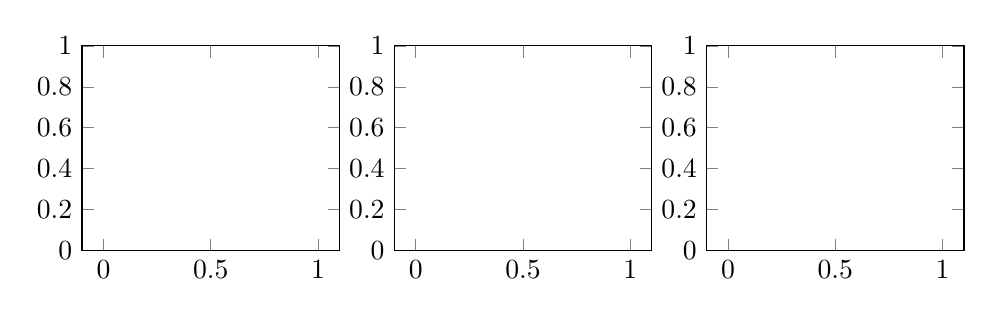
\begin{tikzpicture}

    \begin{axis}[%
            name=plot1,
            width=0.4\linewidth,
            ymin=-0.5, 
            ymax=0]
    \end{axis}

    \begin{axis}[%
            name=plot2,
            width=0.4\linewidth,
            at=(plot1.right of south east), anchor=left of south west,
            ymin=-6.5, ymax=0.2]
    \end{axis}

    \begin{axis}[%
            name=plot3,
            width=0.4\linewidth,
            at=(plot2.right of south east), anchor=left of south west,
            ymin=-6.5, ymax=0.2]
    \end{axis}

\end{tikzpicture}